\section{\textit{Troisième Séance}}

\subsection{Montage électronique}
On va connecter le ruban LED au raspberry Pi, en utilisant une carte de prototypage, en suivant le schéma ci-dessous:

\begin{figure}[htbp]
    \centering
    \includegraphics[width=\textwidth]{Figures/LED_tape_circuit.png}
    \caption{Schéma de connexion du ruban LED au Raspberry Pi}
    \label{fig:schema_led_tape_rpi}
\end{figure}

\subsection{Programmation Python}

\subsubsection{Démarrage}

Une fois le montage électronique réalisé, on peut brancher le clavier, la souris, et le câble micro-hdmi au Raspberry Pi.
Puis, on peut brancher le câble d'alimentation pour allumer le Raspberry Pi 5.

Il va s'allumer, ou "booter", et afficher l'écran de sélection de l'utilisateur.
On va sélectionner:
\begin{itemize}
    \item Utilisateur : \textbf{illumine}
    \item Mot de passe : \textbf{illumine}
\end{itemize}

Après quelques secondes, le bureau du Raspberry Pi 5 va s'afficher.
On va ouvrir le terminal (icône noire avec un \textgreater\_ blanc) pour pouvoir taper des commandes,
comme montré sur la figure \ref{fig:rpi_desktop}.

\begin{figure}[ht]
    \centering
    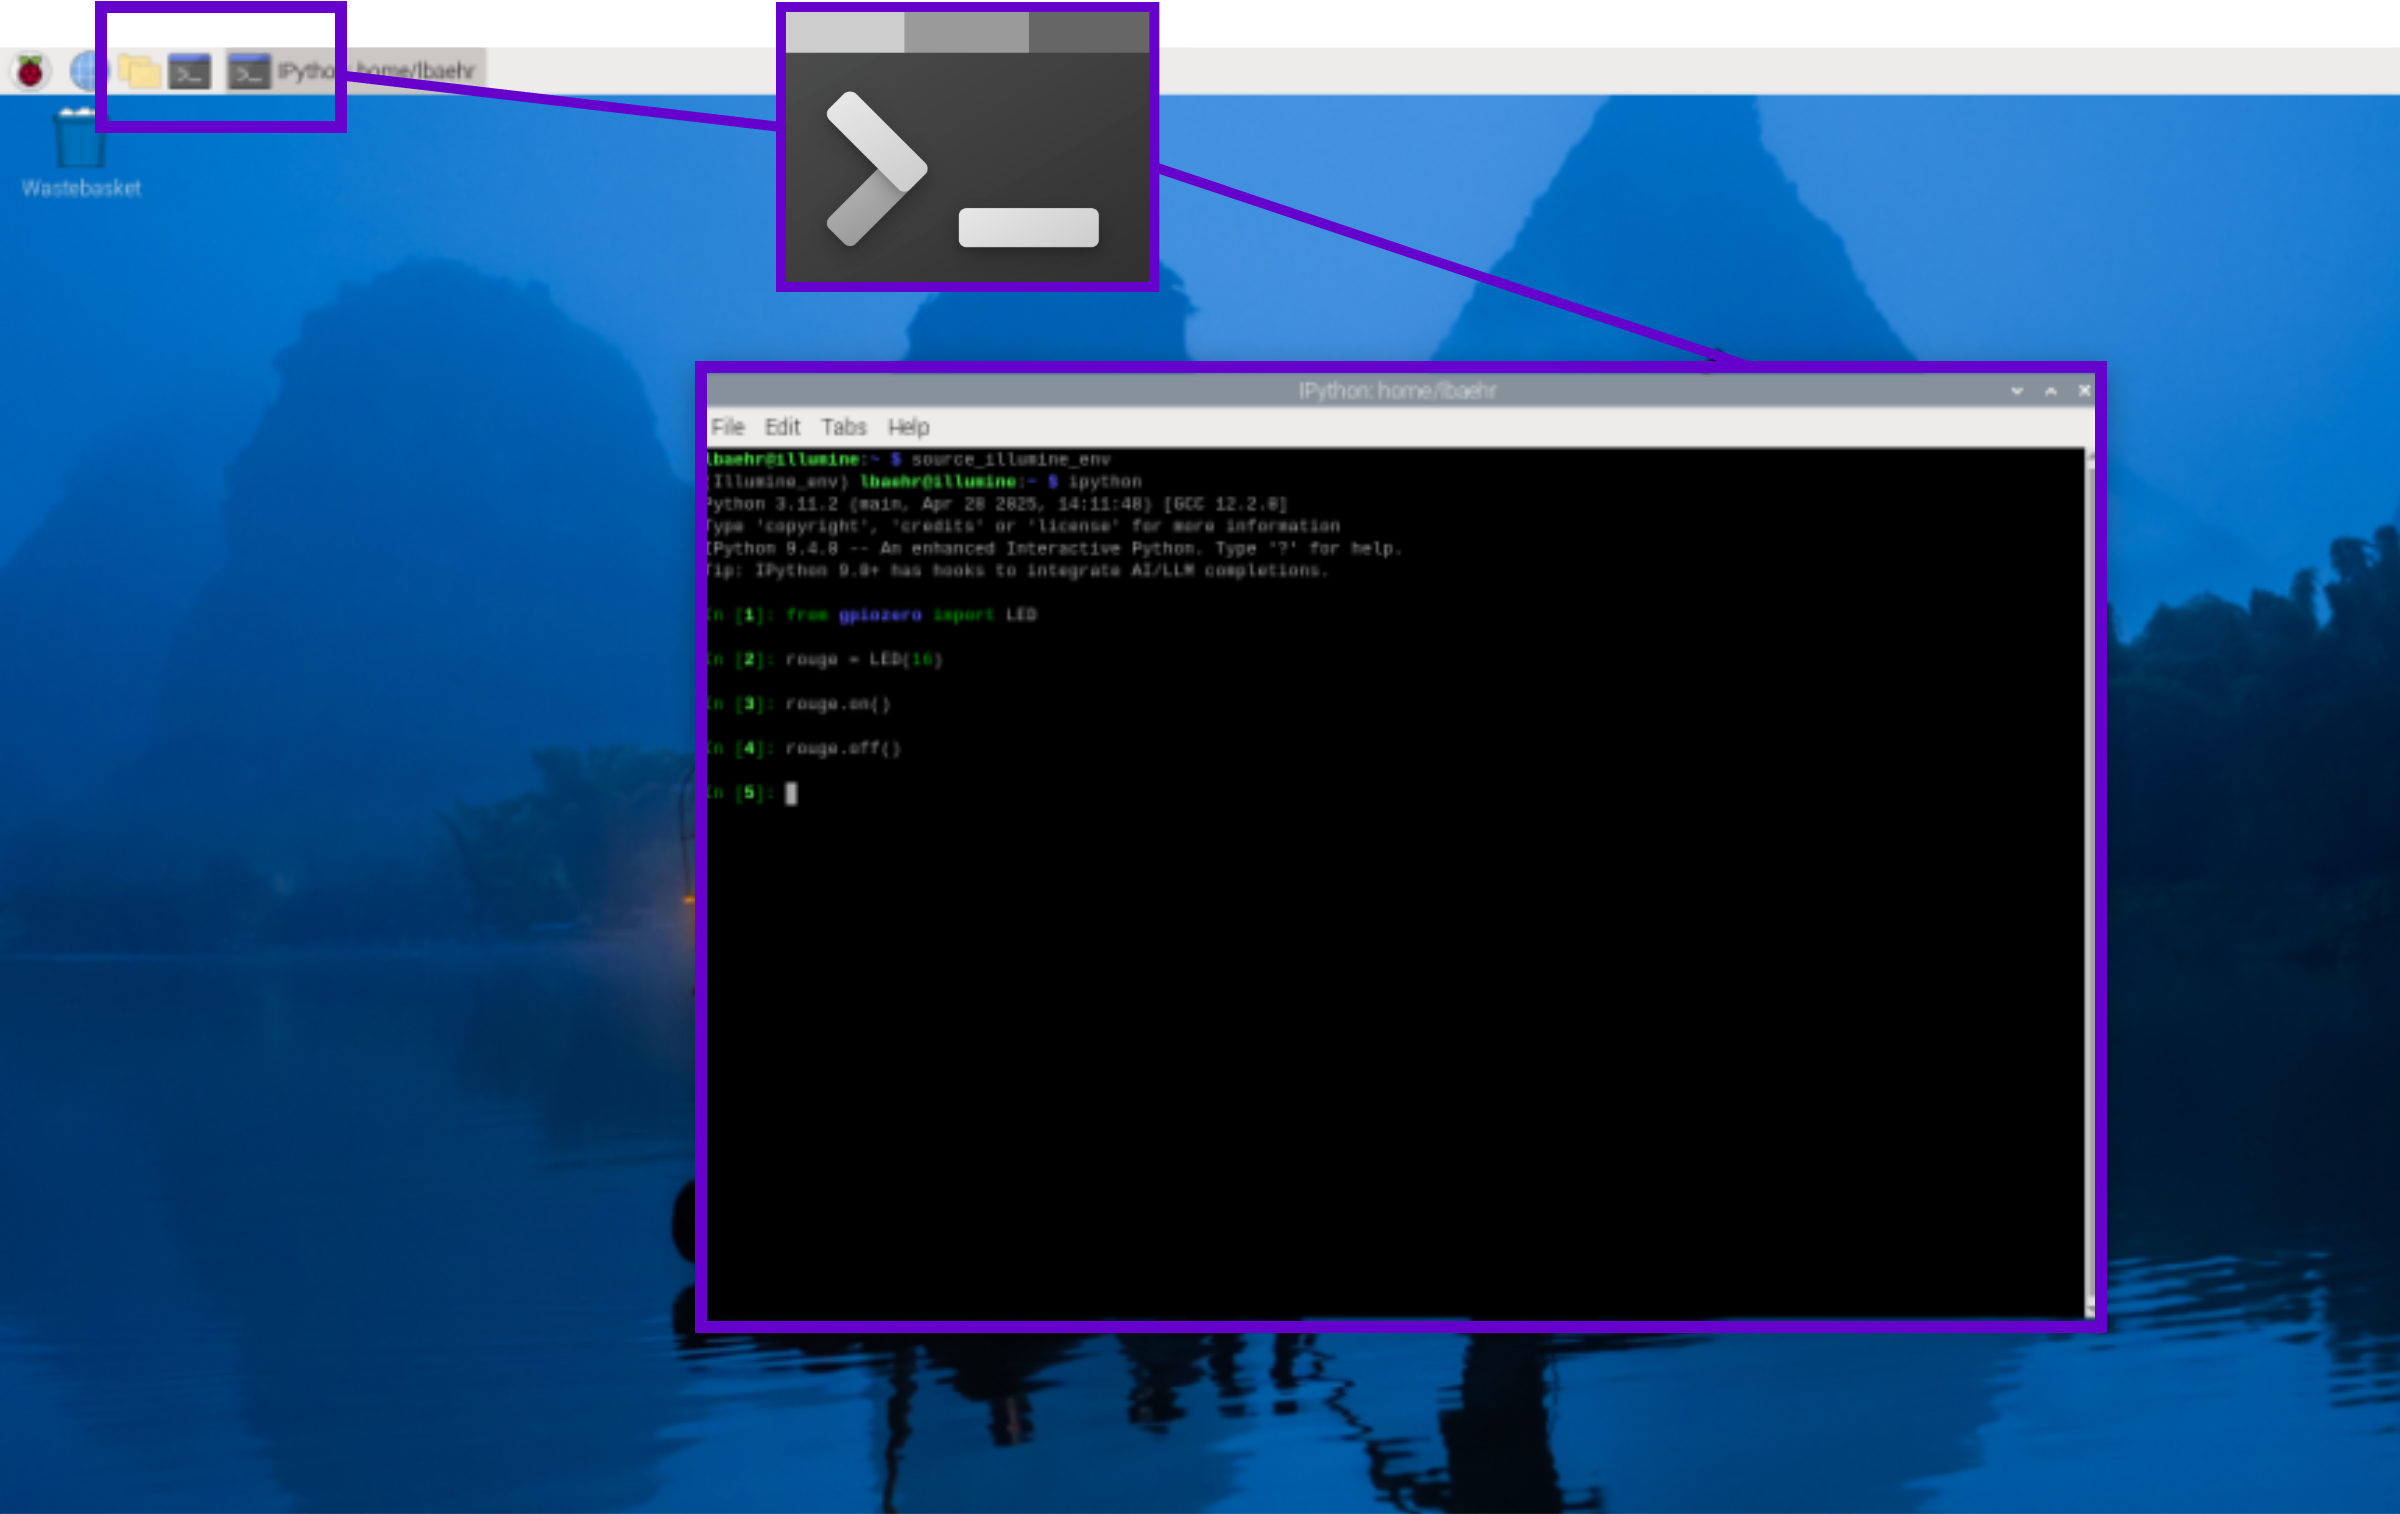
\includegraphics[width=0.8\textwidth]{./Figures/démarrage.png}
    \caption{Bureau du Raspberry Pi 5}
    \label{fig:rpi_desktop}
\end{figure}

\subsubsection{Commandes python}

On va se placer dans un environnement python interactif en tapant les commandes suivantes dans le terminal:
\color{blue}\begin{verbatim}
    cd rpi5_projects/git_repos/illumine/python/3eme_seance/
    source_illumine_env
    ipython
\end{verbatim}
\color{black}

On est maintenant dans un environnement python interactif qui ressemble à celui sur la figure \ref{fig:ipython}.

\begin{figure}[ht]
    \centering
    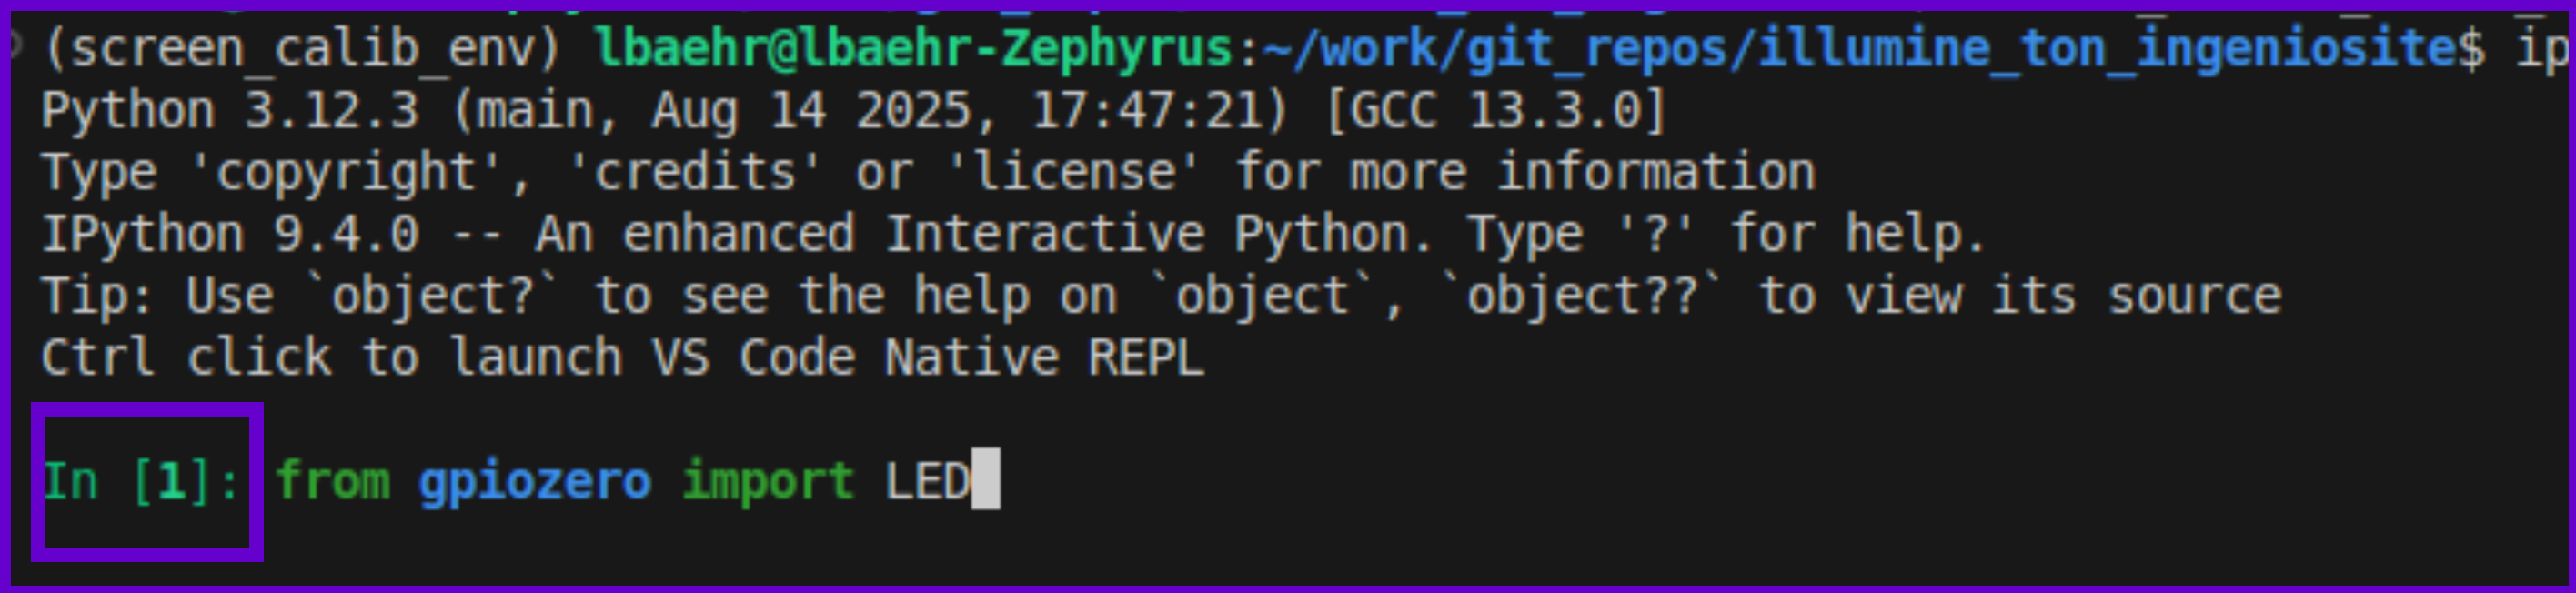
\includegraphics[width=0.8\textwidth]{./Figures/ipython.png}
    \caption{Environnement python interactif}
    \label{fig:ipython}
\end{figure}

On peut donc taper des commandes pour contôler le ruban LED:
\color{blue}\begin{verbatim}
    import RPi5_Neopixel as np 
    ruban = np.Neopixel_Tape()
\end{verbatim}
\color{black}

\subsubsection{Rappel des couleurs disponibles}

Il faut donner un nom de couleur en anglais, alors voici la liste des couleurs disponibles:

\color{blue}
\begin{multicols}{3}
\begin{verbatim}
    'red'
    'dark_red'
    'red_orange'
    'crimson'
    'rust'
    'blood_red'
    'tomato'
    'reddish_orange'
    'burnt_orange'
    'pumpkin'
    'orange'
    'dark_orange'
    'golden_orange'
    'yellow_orange'
    'yellow'
    'bright_yellow'
    'lemon_yellow'
    'pale_yellow'
    'lime_yellow'
    'chartreuse'
    'spring_green'
    'light_green'
    'green'
    'dark_green'
    'forest_green'
    'teal_green'
    'teal'
    'bright_turquoise'
    'medium_turquoise'
    'dark_turquoise'
    'cyan'
    'light_cyan'
    'aqua'
    'light_sky_blue'
    'cornflower_blue'
    'steel_blue'
    'dodger_blue'
    'light_blue'
    'powder_blue'
    'cadet_blue'
    'lavender_blue'
    'light_indigo'
    'indigo'
    'blue_violet'
    'purple'
    'medium_purple'
    'orchid'
    'violet'
    'thistle_purple'
    'pink_purple'
    'magenta'
    'fuchsia'
    'hot_pink'
    'light_pink'
    'pink'
    'light_coral'
    'salmon_pink'
    'coral'
    'tomato_pink'
    'rosy_brown'
\end{verbatim}
\end{multicols}
\color{black}

N'oublie pas les guillements autour du nom de la couleur !

\subsubsection{Rappel des fonctions élémentaires et nouvelles fonctions}

Plusieurs fonctions élémentaires sont disponibles pour piloter une ou plusieurs LED du ruban. Voici un rappel
de ce qu'elles permettent de faire. \par

\color{blue}
\texttt{ruban.on\_led(num, color\_name)} : \color{black} Allume la LED numéro \texttt{num} avec la couleur \texttt{color\_name}. \par
\vspace{1em}
\color{blue}\texttt{ruban.off\_led(num)} : \color{black} Éteint la LED numéro \texttt{num}. \par
\vspace{1em}
\color{blue}\texttt{ruban.on\_all\_led(color\_name)} : \color{black} Allume toutes les LED avec la couleur \texttt{color\_name}. \par
\vspace{1em}
\color{blue}\texttt{ruban.off\_all\_led()} : \color{black} Éteint toutes les LED. \par
\vspace{1em}
\color{blue}\texttt{ruban.recule(num, color\_name, times)} : \color{black} Fait reculer une lumière de couleur \texttt{color\_name} à partir de la LED numéro \texttt{num}, pendant \texttt{times} étapes. \par
\vspace{1em}
\color{blue}\texttt{ruban.clignote(num, color\_name, times)} : \color{black} Fait clignoter la LED numéro \texttt{num} de couleur \texttt{color\_name}, \texttt{times} fois. \par
\vspace{1em}
\color{blue}\texttt{ruban.clignote\_all(color\_name, times)}\ : \color{black} Fait clignoter toutes les LED de couleur \texttt{color\_name}, \texttt{times} fois.\ \par
\vspace{1em}
\color{blue}\texttt{ruban.random(color\_name, times)}\ : \color{black} Allume des LED aléatoires de couleur \texttt{color\_name}, \texttt{times} fois.\ \par
\vspace{1em}

\paragraph{Nouvelles fonctions}
Des fonctions plus complexes sont aussi disponibles, à toi de les tester pour voir ce qu'elles font ! \par

\textit{Exercice:} Essaye les fonctions suivantes en remplaçant \textbf{num} par un numéro de LED entre 0 et 59,
\vspace{1em}
\textbf{color\_name} par un nom de couleur de la liste précédente, et \textbf{times} par le nombre de fois
que tu veux faire l'effet.
Décris sur les pointillés ce que fait chaque fonction.

\color{blue}
\begin{verbatim}
    ruban.charge(color_name, times): ............................................

    ruban.chariot(color_name, times): ...........................................

    ruban.deux_chariots(color_name, times): .....................................

    ruban.croise(color_name, times): ............................................
\end{verbatim}
\color{black}

\subsubsection{Arc-en-ciel en mouvement}
\label{sec:arc_en_ciel}

Nous allons maintenant écrire un script pour créer un arc-en-ciel en mouvement. Pour cela, nous allons utiliser
la fonction suivante:
\vspace{1em}

\color{blue}\texttt{ruban.fill\_rainbow(shift)}\ : \color{black} Remplit le ruban avec un dégradé de couleurs arc-en-ciel. Si \texttt{shift=0} alors la première LED sera rouge
mais si \texttt{shift=1} alors la première LED sera de la couleur de la dernière LED précédente, c'est à dire rose.
Si \texttt{shift=5} alors la première LED sera rose-violet, et ainsi de suite. \textbf{On voit que \texttt{shift} décale
l'arc-en-ciel!}\par

\vspace{1em}

On va maintenant quitter l'environnement python interactif en tapant la commande \color{blue}
\texttt{exit()} \color{black}.

\textit{Exercice:} Tape la commande suivante pour ouvrir et compléter le script python \texttt{rainbow\_cycle.py}:

\color{blue}
\begin{verbatim}
    gedit rainbow_cycle.py
\end{verbatim}
\color{black}

Une fenêtre comme celle de la figure \ref{fig:rainbow} va s'ouvrir. Efface les symboles \texttt{\#\#\#}
et remplace-les par une boucle \texttt{for} qui fait varier \texttt{\textbf{i}}~dans~\texttt{\textbf{range(num\_pixels)}},
et par \texttt{fill\_rainbow} avec \texttt{shift=i} pour faire un arc-en-ciel en mouvement\!

\begin{figure}[ht]
    \centering
    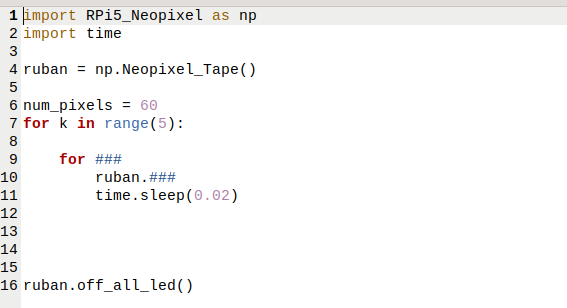
\includegraphics[width=0.8\textwidth]{./Figures/rainbow.png}
    \caption{Fonction rainbow\_cycle.py à compléter}
    \label{fig:rainbow}
\end{figure}

Une fois terminé, sauvegarde le fichier (Ctrl+S), et tu peux soit fermer la fenêtre et revenir au terminal, soit
garder la fenêtre ouverte, ouvrir un autre terminal et retaper:
\color{blue} 
\begin{verbatim} 
    cd rpi5_projects/git_repos/illumine/python/3eme_seance/
    source_illumine_env
\end{verbatim}
\color{black} 

Dans les deux cas, tape:
\color{blue}
\begin{verbatim}
    python3 rainbow_cycle.py
\end{verbatim}
\color{black}
pour exécuter ton script python et voir si le résultat est celui attendu !

\subsection{Faire sa propre démo !}

Regarde ce que fait la commande:
\color{blue}\begin{verbatim}
    python3 demo_ruban.py
\end{verbatim}
\color{black}

On voit ouvrir ce script pour que tu puisses le modifier et faire ta propre démo !

\color{blue}\begin{verbatim}
    gedit demo_ruban.py
\end{verbatim}
\color{black}

Utilise les fonctions en exemple dans le script mais aussi toutes celles qu'on a vu précédemment. 
Ajoute bien des \color{blue}\texttt{time.sleep(0.1)}\color{black} entre les commandes pour que les effets soient visibles.

\subsection{Éteindre le Raspberry Pi 5}

On peut éteindre le RPi 5 comme un ordinateur classique, mais on peut aussi l'éteindre avec
une commande dans le terminal:

\color{blue}\begin{verbatim}
    sudo shutdown -h now
\end{verbatim}

\color{black}

Il faut taper le mot de passe: rien ne s'affiche quand tu tapes mais c'est normal !
Tape le bon mot de passe et le RPi 5 va s'éteindre.

Bravo !